\chapter{Algoritmo di back-propagation} % (fold)
\label{cha:algoritmo_di_back_propagation}
Il problema incontrato nell’addestramento delle reti multistrato è il seguente: volendo adottare un meccanismo di aggiornamento dei pesi simile a quello nelle reti a singolo strato (in cui l’errore è calcolato come differenza tra l’uscita desiderata e l’uscita effettiva di ciascun neurone) si riesce ad aggiornare solo i pesi relativi ai neuroni di uscita, ma non quelli relativi ai neuroni degli strati nascosti. Infatti, mentre per lo strato di uscita si conosce l’uscita desiderata (tale uscita viene data come secondo elemento delle coppie che costituiscono gli esempi del training set), niente si sa dell’uscita desiderata dai neuroni nascosti.\\

Questo problema è stato risolto dopo molti anni di disinteresse per le reti neurali (in quanto non si riusciva ad addestrarle) solo nel 1986, quando fu introdotto l’algoritmo di backpropagation. Tale algoritmo prevede di calcolare l’errore commesso da un neurone dell’ultimo strato nascosto propagando all’indietro l’errore calcolato sui neuroni di uscita collegati a tale neurone. Lo stesso procedimento è poi ripetuto per tutti i neuroni del penultimo strato nascosto, e così via.\\

L’algoritmo di backpropagation prevede che, per ogni esempio del training set, i segnali viaggino dall’ingresso verso l’uscita al fine di calcolare la risposta della rete. Dopo di che c’è una seconda fase durante la quale i segnali di errore vengono propagati all’indietro, sulle stesse connessioni su cui nella prima fase hanno viaggiato gli ingressi, ma in senso contrario, dall’uscita verso l’ingresso. Durante questa seconda fase vengono modificati i pesi.\\

I pesi sono inizializzati con valori casuali. Come funzione di uscita non lineare dei neuroni della rete si adotta in genere la funzione sigmoidea (l’algoritmo richiede che la funzione sia derivabile). L'algoritmo è basato sul metodo della \textbf{discesa del gradiente}.

\section{Metodo di discesa del gradiente} % (fold)
\label{sec:metodo_di_discesa_del_gradiente}

Il gradiente di una funzione $f$, denotato con $\nabla f$ è il vettore che ha come componenti le derivate parziali della funzione.
\begin{align}
    \nabla f(\bar{x}) = \left( \frac{\partial f(\bar{x})}{\partial x_1}, \frac{\partial f(\bar{x})}{\partial x_2}, \dots, \frac{\partial f(\bar{x})}{\partial x_n} \right)
\end{align}

La discesa del gradiente è una tecnica di ottimizzazione di tipo locale. Consiste nel valutare, inizialmente in un punto scelto a caso nello spazio multidimensionale (primo punto), sia la funzione stessa sia il suo gradiente.\\

Il gradiente indica la direzione in cui la funzione tende a un minimo/massimo, ovvero dove il gradiente tende a 0. Se si è interessati alla ricerca di un \textbf{minimo locale} si considerano i passi proporzionali al \emph{negativo} del gradiente della funzione nel punto corrente. Se, invece, si prendono i passi proporzionali al \emph{positivo} del gradiente si raggiungerà un \textbf{massimo locale}; la procedura in questo caso è nota come \emph{ascesa del gradiente}.\\

A titolo di esempio, il gradiente di $f(x, y) = x^2 + xy$ è:
\begin{align*}
    \nabla f(x, y) = \left\{\frac{df}{dx}, \frac{df}{dy} \right\} = \{2x + y, x\}
\end{align*}

% section metodo_di_discesa_del_gradiente (end)


\section{Apprendimento supervisionato} % (fold)
\label{sec:apprendimento_supervisionato}
L'algoritmo di backpropagation è un algoritmo di \emph{apprendimento supervisionato}, che prevede di presentare alla rete per ogni esempio di addestramento la corrispondente uscita desiderata.\\

Di solito i pesi vengono inizializzati con valori casuali all’inizio dell’addestramento. Poi si cominciano a presentare, uno alla volta, gli esempi costituenti l’insieme di addestramento (training set). Per ogni esempio presentato si calcola l’errore commesso dalla rete, cioè la differenza tra l’uscita desiderata e l’uscita effettiva della rete. L’errore è usato per aggiustare i pesi.\\

Il processo viene di solito ripetuto ripresentando alla rete, in ordine casuale, tutti gli esempi del training set finchè l’errore commesso su tutto il training set (oppure l’errore medio sul training set) risulta inferiore ad una soglia prestabilita.

\newpage

Dopo l’addestramento la rete viene testata controllandone il comportamento su un insieme di dati, detto test set, costituito da esempi non utilizzati durante la fase di training. La fase di test ha quindi lo scopo di valutare la capacità di generalizzazione della rete neurale.
Si dice che la rete ha imparato, cioè è in grado di fornire risposte anche per ingressi che non le sono mai stati presentati durante la fase di addestramento.\\

Ovviamente le prestazioni di una rete neurale dipendono fortemente dall’insieme di esempi scelti per l’addestramento. Tali esempi devono quindi essere rappresentativi della realtà che la rete deve apprendere e in cui verrà utilizzata. L’addestramento è in effetti un processo ad hoc dipendente dallo specifico problema trattato.\\

Tecnicamente, è necessario un insieme di addestramento $L$ della forma: 
\begin{align}
    L = \{(\bar{x}_1, \bar{y}_1), \dots, (\bar{x}_p, \bar{y}_p) \}
\end{align}
dove
\begin{align*}
    &\bar{x}_\mu \mbox{ con $\mu=1, \dots, p$ è il vettore input} \\
    &\bar{y}_\mu \mbox{ con $\mu=1, \dots, p$ è il vettore dell'output desiderato}
\end{align*}

L'apprendimento consiste nel trovare una configurazione di pesi in modo tale che l'output della rete sia il più vicino possibile all'output desiderato per tutti gli esempi presenti nel training set.\\

Formalmente, si tratta di trovare una configurazione di pesi tra tutte le possibili combinazioni $\overline{W}$ che minimizzi la seguente \emph{funzione di errore}. Essa dipende dal vettore h-esimo di output $out_\mu$ restituito dalla rete, dato il vettore $\mu$-esimo di ingresso $\overline{x}_\mu$ e dal vettore h-esimo di output $\overline{y}_\mu$ del training set. In termini matematici:
\begin{align*}
    \min_{\bar{w} \in \overline{W}} E(\bar{w}) &= \frac{1}{2} \sum_{\mu=1}^p \| \underbrace{\bar{y}_\mu}_\textrm{desiderato} - \underbrace{out_\mu (\bar{w})}_\textrm{reale} \|_2^2 \\
    &= \frac{1}{2} \sum_{\mu=1}^p \sum_{k=1}^n \left(y_k^\mu - out_k^\mu (\bar{w})\right)^2
\end{align*}
dove l'indice $k$ rappresenta il valore corrispondente al k-esimo neurone di output e il termine $1/2$ è aggiunto per cancellare l'esponente durante la derivazione.
% section apprendimento_supervisionato (end)

\newpage

\section{Propagazione dell'errore} % (fold)
\label{sec:back_propagation}
La funzione $E$ è altamente non lineare pertanto il problema di ottimizzazione non è facile da risolvere. Per minimizzare la funzione si utilizza il metodo della discesa del gradiente. Per calcolare le derivate parziali $\partial E / \partial w_{ij}$ è necessario l'algoritmo di back propagation. L'algoritmo può essere diviso in due passi:
\begin{itemize}
    \item \emph{Forward pass:} l'input dato alla rete è propagato al livello successivo e così via ai livelli successivi (il flusso di informazioni si sposta in avanti, cioè forward). Si calcola dunque $E(\bar{w})$, l'errore commesso.
    \item \emph{Backward pass:} L'errore fatto dalla rete è propagato all'indietro (backward) e i pesi sono aggiornati in maniera appropriata.
\end{itemize}
Il seguente schema descrive il funzionamento dell'algoritmo di retroazione.
\begin{figure}[h!]
    \centering
    \begin{tikzpicture}[->,shorten >=2pt, shorten <= 2pt, auto, node distance=\layersep]
        \def\nodesep{-2cm}
        \def\layersep{4cm}
        % Draw the input layer nodes
        \foreach \name / \y in {1,...,4}
            \node[input neuron, pin=left:$x_\y$] (I-\name) at (0, \nodesep * \y) {};

        % Draw the hidden layer nodes
        \foreach \name / \y in {1,...,3}   
            \node[hidden neuron, pin={[pin edge={->}] above:$V_\y$}] (H-\name) at (\layersep, \nodesep * \y - 1 cm) {};
            
        % Draw the output layer nodes
        \foreach \name / \y in {1,...,2}   
            \node[output neuron, pin={[pin edge={->}]right:$O_\y$}] (O-\name) at (2*\layersep, \nodesep * \y - 2cm) {};

        % Connect every node in the input layer with every node in the hidden layer.
        \foreach \source in {1,...,4}
            \foreach \dest in {1,...,3}
                \path (I-\source) edge (H-\dest);

        % Error edges.
        \foreach \source in {1,...,4}
            \foreach \dest in {1,...,3}
                \path (H-\dest) edge[dashed, color=blue, transform canvas={yshift=1mm}] (I-\source);

        \foreach \source in {1,...,3}
            \foreach \dest in {1,...,2}
                \path (O-\dest) edge[dashed, color=blue, transform canvas={yshift=1mm}] (H-\source);


        \path (I-1) edge[above] node {$w_{11}$} (H-1);
        \path (I-4) edge[below] node {$w_{34}$} (H-3);
        % Connect every node in the hidden layer with every node in the output layer.
        \foreach \source in {1,...,3}
            \foreach \dest in {1,...,2}
                \path (H-\source) edge (O-\dest);


        \path (H-1) edge[above] node {$W_{11}$} (O-1);
        \path (H-3) edge[below] node {$W_{23}$} (O-2);
        
        % Annotate the layers
        \node[annot,above of=H-1, node distance=2cm] (hl) {Hidden layer};
        \node[annot,left of=hl] {Input layer};
        \node[annot,right of=hl] {Output layer};
        
        \node at (-1.3, - 9) {$x_k$};
        \node at (2, - 9) {$w_{jk}$};
        \node at (4, - 9) {$V_j$};
        \node at (6, - 9) {$W_{ij}$};
        \node at (9.3, - 9) {$O_i$};
        
    \end{tikzpicture}
    \caption{Schema back-propagation: le linee nere indicano il segnale propagato in avanti, mentre quelle blu indicano l'errore propagato all'indietro.}\label{fig:backpro}
\end{figure}

Considereremo un metodo semplice che aggiorna i pesi di pattern in pattern fino al raggiungimento di un'epoca. \textbf{Un'epoca} è un ciclo di presentazione di tutti gli esempi del training set.
L'aggiustamento dei pesi viene fatto in base all'errore calcolato per ogni pattern presentato alla rete.
\newpage

Si definiscono ora, in termini matematici, gli input e gli output prodotti dai neuroni nascosti e di output.
Dato un pattern $\mu$, l'unità nascosta $j$ riceve un input netto dato da:
\begin{align}
    h_j^\mu = \sum_k w_{jk} x^\mu_k
\end{align}
e produce come output:
\begin{align}
    V_j^\mu = g(h_j^\mu) = g\left(\sum_k w_{jk} x^\mu_k \right)
\end{align}
Dove $g$ è la funzione di attivazione. In modo analogo il segnale entrante nell'unità output $i$ è definito come:
\begin{align}
    h_i^\mu = \sum_j W_{ij} \cdot V^\mu_j
\end{align}
E l'output prodotto $O_i$ è:
\begin{align}
    O_i = g(h^\mu_i) = g\left(\sum_j W_{ij} V^\mu_j \right)
\end{align} 
I pesi sono aggiornati nella direzione opposta rispetto al gradiente; siamo infatti interessati a trovare un minimo per la funzione $E$. Quindi i pesi all'iterazione $t + 1$ sono così calcolati:
\begin{align*}
    w^{t+1} = w^t - \eta \cdot \nabla (E(w^t))
\end{align*}


Il parametro $\eta$ noto come \textbf{fattore di apprendimento} ha una forte influenza sul comportamento dell'algoritmo (velocità di convergenza, oscillazioni, ecc..).

\begin{figure}[h!]
    \centering
    \begin{tikzpicture}
        \node[draw,circle,inner sep=1pt,fill] (1) at (0, 0) {};
        \node[above right=1mm of 1] {$w^t$};
        \node[draw,circle,inner sep=1pt,fill] (2) at (2, -1) {};
        \node[above right=1mm of 2] {$w^{t+1}$};
        \node (3) at (4, -2) {};
        \draw[->] (2) -- (3);
        \node[below=0.1mm of 3] {$-\nabla (E(w^t))$};
        \path (1) edge[very thick, below] node {$\eta$} (2);
    \end{tikzpicture}
    \caption{Direzione di aggiornamento dei pesi.}
\end{figure}

\newpage

\subsection{Aggiornamento pesi strato nascosto-output} % (fold)
\label{sub:aggiornamento_pesi_strato_nascosto_output}

Calcoliamo ora la variazione di peso sinaptico tra il neurone di output $i$ e il neurone nascosto $j$ per un certo pattern $\mu$ del training set. Da notare come nella Figura~\ref{fig:backpro} utilizziamo la $W$ maiuscola per indicare i pesi tra il layer nascosto e quello ouput.
\begin{align*}
    \Delta W_{ij} &= - \eta \cdot \frac{\partial E}{\partial W_{ij}} \\
    &= - \eta \cdot \frac{\partial}{\partial W_{ij}}\left[\frac{1}{2} \sum_\mu \sum_k (y_k^\mu - O_k^\mu)^2 \right]\\
    &= - \eta \cdot \sum_\mu \sum_k (y_k^\mu -O_k^\mu) \cdot \left( -  \frac{\partial O_k^\mu} {\partial W_{ij}} \right) = \eta \cdot \sum_\mu \sum_k (y_k^\mu -O_k^\mu) \frac{\partial O_k^\mu}{\partial W_{ij}} \\
    &\text{Per $k\neq i$, $O_k$ non dipende da $W_{ij}$, quindi la derivata per $O_k$ è 0;} \\
    &\text{ad esempio vedi Figura~\ref{fig:backpro} il peso $W_{11}$ non influenza $O_2$. } \\
    &= \eta \cdot \sum_\mu  (y_i^\mu - O_i^\mu) \frac{\partial O_i^\mu}{\partial W_{ij}} \\
    &= \eta \cdot \sum_\mu  (y_i^\mu - O_i^\mu) \cdot g'(h_i^\mu) \cdot \frac{\partial h_i^\mu}{\partial{W_{ij}}}
\end{align*}
Calcoliamo la derivata di $\partial h_i^\mu / \partial W_{ij}$:
\begin{align*}
    \frac{\partial h_i^\mu}{\partial{W_{ij}}} &= \frac{\partial}{\partial{W_{ij}}} \sum_l V_l^\mu \cdot W_{il} \\
    & \text{Come prima per $l\neq j$ la derivata di $h^\mu_i$ è 0} \\
    &= \frac{\partial}{\partial{W_{ij}}} V_j^\mu \cdot W_{ij} = V_j^\mu
\end{align*}
Quindi:
\begin{align*}
    \Delta W_{ij} = \eta \cdot \sum_\mu  (y_i^\mu - O_i^\mu) \cdot g'(h_i^\mu) \cdot V_j^\mu = \eta \cdot \sum_\mu \delta^\mu_i V^\mu_j
\end{align*}
Dove:
\begin{align*}
    \delta^\mu_i = (y^\mu_i - O^\mu_i) g'(h^\mu_i)
\end{align*}
è l'errore del neurone $i$-esimo ed è noto come \textbf{gradiente locale}.
% subsection aggiornamento_pesi_strato_input_nascosto (end)
\newpage

\subsection{Aggiornamento pesi strato input-nascosto} % (fold)
\label{sub:aggiornamento_pesi_strato_input_nascosto}
Passiamo ora al calcolo della variazione di peso sinaptico tra il neurone nascosto $j$ e il neurone di input $k$ per un certo pattern $\mu$ del training set.
\begin{align*}
    \Delta w_{jk} &= - \eta \cdot \frac{\partial E}{\partial w_{jk}} \\
    &= \eta \cdot \sum_\mu \sum_i (y^\mu_i - O^\mu_i)  \frac{\partial O^\mu_i}{\partial w_{jk}} \\
    &= \eta \cdot \sum_\mu \sum_i (y^\mu_i - O^\mu_i) \cdot   g'(h^\mu_i) \frac{\partial h^\mu_i}{\partial w_{jk}}
\end{align*}
In questo caso la seconda sommatoria rimane in quanto l'output dipende indirettamente dall'input; ad esempio il segnale entrante in $O_1$ dipende indirettamente da $w_{jk}$.
Calcoliamo ora $\partial h^\mu_i / \partial w_{jk}$:
\begin{align*}
    \frac{\partial h^\mu_i}{\partial w_{jk}} &= \sum_l W_{il} \frac{\partial V_l^\mu}{\partial w_{jk}} \\
    &\text{Come prima per $l\neq j$, $V_l$ non dipende da $w_{jk}$.} \\
    &= W_{ij} \frac{\partial V_j^\mu}{\partial w_{jk}} \\
    &= W_{ij} \frac{\partial g(h^\mu_j)}{\partial w_{jk}} \\
    &= W_{ij} g'(h^\mu_j) \frac{\partial h^\mu_j}{\partial w_{jk}}
\end{align*}
La derivata di $\partial h^\mu_j / \partial w_{jk}$ è:
\begin{align*}
	\frac{\partial h^\mu_j}{\partial w_{jk}} 
	&= \frac{\partial}{\partial w_{jk}} \sum_m w_{jm} x^\mu_m \\
	&\text{Come al solito per $m \neq k$ la derivata è 0.} \\
	&= \frac{\partial}{\partial w_{jk}} w_{jk} x^\mu_k\\
	&= x^\mu_k
\end{align*}

\newpage

Quindi abbiamo:
\begin{align*}
    \Delta w_{jk} &= \eta \cdot \sum_\mu \sum_i (y_i^\mu - O^\mu_i) \cdot g'(h^\mu_i) W_{ij} g'(h_j^\mu) x^\mu_k\\
    &= \eta \cdot \sum_\mu \sum_i \delta_i^\mu W_{ij} g'(h_j^\mu) x^\mu_k \\
    &= \eta \cdot \sum_\mu \hat{\delta}_j^\mu x^\mu_k
\end{align*}
% subsection aggiornamento_pesi_strato_nascosto_output (end)

Dove:
\begin{align*}
    \hat{\delta}_j^\mu = g'(h_j^\mu) \sum_i \delta^\mu_i W_{ij}
\end{align*}
è il gradiente locale del neurone nascosto $j$ e la sommatoria rappresenta l'errore medio sullo strato di output causato dal neurone $j$ dello strato nascosto.

\newpage

\subsection{In generale} % (fold)
\label{ssub:in_generale}
\begin{figure}[h!]
    \centering
    \begin{tikzpicture}
        \node[draw, circle] (1) at (0, 0) {$p$};
        \node[above=1mm of 1] {$\delta_p^\mu$};
        \node[draw, circle] (2) at (4, -1){$q$};
        \node[above=1mm of 2] {$V_q^\mu$};
        
        \path (1) edge[<-, thick, midway, above] node {$w_{pq}$} (2);
        
    \end{tikzpicture}
    \caption{Variazione di peso sinaptico.}
\end{figure}

In generale per l'aggiornamento dei pesi non sono necessarie informazioni globali, ma solo locali. La variazione di peso sinaptico tra un neurone $p$ e $q$ relativo ad un pattern $\mu$ del training set è dato da:
\begin{align}
    \Delta w_{pq} = \eta \, \delta^\mu_p \, V^\mu_q
\end{align}
Dove:
\begin{align*}
    \delta_p^\mu =
    \begin{cases}
        (y^\mu_p - O^\mu_p) \, g'(h^\mu_p), &\text{se $p$ è un neurone di ouput} \\
        \displaystyle g'(h_p^\mu) \, \sum_i \delta^\mu_i \, W_{ip} &\text{altrimenti}
    \end{cases}
\end{align*}
Questo modello prende il nome di apprendimento \textbf{on-line} in quanto la rete apprende un esempio alla volta. Esiste però un altro modello detto \textbf{off-line} o batch che considera tutti gli esempi dell'insieme di addestramento alla volta, anche se questo è meno coerente al modello biologico. Per l'apprendimento off-line abbiamo la seguente regola di apprendimento:
\begin{align}
    \Delta w_{pq} = \eta \, \sum_\mu \delta^\mu_p \, V^\mu_q
\end{align}

% subsection in_generale (end)
% section back_propagation (end)

\newpage

\section{I passi dell'algoritmo} % (fold)
\label{sec:l'algoritmo}

\algrenewcommand{\alglinenumber}[1]{\scriptsize\circled{#1}}% circled line numbers
Si consideri una rete con $M$ strati e $m=0,\dots,M$. Si denota inoltre
\begin{itemize}
    \item $V^m_i$: output della i-esima unità del livello m;
    \item $w^{ij}_m$: peso della connessione tra il j-esimo neurone dello strato $m-1$ e l'i-esimo neurone dello strato $m$. 
\end{itemize}
L'algoritmo di retroazione si compone dei seguenti passi:
\begin{algorithmic}[1]% Taken from the algorithmicx package documentation
    \State Inizializzazione dei pesi a (piccoli) valori casuali;
    \State Scelta di un pattern $\overline{x}^\mu$ da inserire allo strato input $(m=0)$:
    \begin{align*}
        V^0_k = x^\mu_k \qquad \forall k
    \end{align*}
    \State Propagazione del segnale in avanti:
    \begin{align*}
        V^m_i = g(h_i^m) = g\left(\sum_j w_{ij} V_j^{m-1}\right)
    \end{align*}
    \State Calcolo degli errori $\delta$ dello strato output;
    \begin{align*}
        \delta^M_i = (y^M_i - V^M_i) \, g'(h^M_i)
    \end{align*}
    \State Calcolo degli errori $\delta$ per tutti gli strati precedenti;
    \begin{align*}
        \delta^{m-1}_i = g'\left(h^{m-1}_i\right) \, \sum_j \delta^m_j \, W_{ji}
    \end{align*}
    \State Aggiornamento dei pesi;
    \begin{align*}
        w^{NEW}_{ij} = w^{OLD}_{ij} + \Delta w_{ij} \qquad \text{dove } \Delta w_{ij} = \eta \delta_i^m V_j^{m-1} 
    \end{align*}
    \State Torna al passo 2 fino alla convergenza.
\end{algorithmic}
L'algoritmo si potrebbe fermare quando $\| w^{t+1} - w^t \| < \epsilon$ oppure dopo un certo numero di epoche se la condizione precedente non è rispettata.

\newpage

% section i_passi_dell'algoritmo (end)

\section{Il momento} % (fold)
\label{sub:il_momento}
La scelta di $\eta$ influenza molto il comportamento dell'algoritmo, infatti se scegliamo valori troppo piccoli, la convergenza sarà lenta, mentre se scegliamo valori troppo grandi si rischia di avere una rete instabile con comportamento oscillatorio.
Un metodo semplice per incrementare il fattore di apprendimento senza il rischio di rendere la rete instabile consiste nel modificare la regola di aggiornamento inserendo un nuovo termine: \emph{il momento}, una costante di proporzionalità alla precedente variazione dei pesi.
\begin{align}
    \Delta w_{pq} (t + 1) = \underbrace{\alpha \Delta_{pq} (t)}_\textrm{momento} - \eta \frac{\partial E}{\partial w_{pq}}
\end{align}
Dove $\alpha$ è un numero positivo a scelta preferibilmente compreso in $[0,1)$. In questo modo, il cambiamento dei pesi per l’esempio $t+1$ dipende dal cambiamento apportato ai pesi per l’esempio $t$.
L'utilizzo del momento ha l'effetto di incrementare o decrementare l'ampiezza di aggiornamento in modo tale da \textbf{accellerare nelle discese} o \textbf{stabilizzare} l'algoritmo in caso di oscillazioni. Questo fatto ha, inoltre, il vantaggio di \textbf{prevenire} (non con certezza) che il processo di apprendimento incappi in minimi locali della funzione d'errore.

\begin{figure}[h!]
    \centering
    \subfigure[Assenza di momento $\alpha=0$]{
        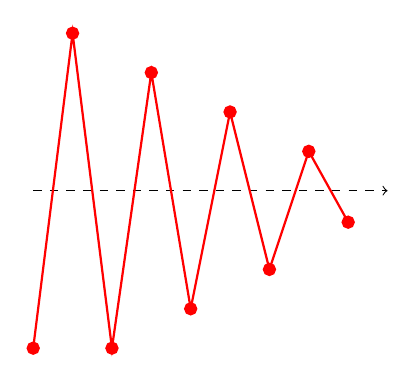
\begin{tikzpicture}
            \draw[->, dashed] (-2,0) -- (2.5,0);
            \draw[thick, color=red] plot [mark=*,red, tension=1.5] coordinates{
            (-2,-2) (-1.5, 2) (-1, -2) (-0.5, 1.5) (0, -1.5) (0.5, 1) (1, -1) (1.5, 0.5) (2, -0.4)};
        \end{tikzpicture}
    }
    \qquad
    \subfigure[Con momento $\alpha=0.5$]{
        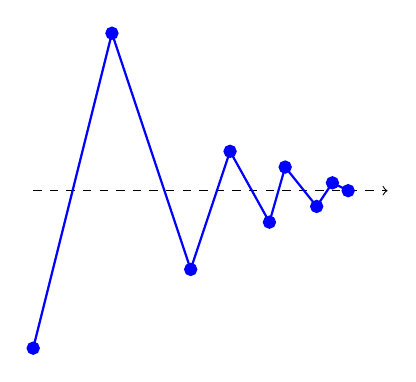
\begin{tikzpicture}
            \draw[->, dashed] (-2,0) -- (2.5,0);
            \draw[thick, color=blue] plot [mark=*,blue, tension=1.5] coordinates{
            (-2,-2) (-1, 2) (0, -1) (0.5, 0.5) (1, -0.4) (1.2, 0.3) (1.6, -0.2) (1.8, 0.1) (2, 0)};
        \end{tikzpicture}
    }
    \caption{Momento e discesa del gradiente su una semplice superficie.}
\end{figure}

% section il_momento (end)

\newpage

\section{Problema del minimo locale} % (fold)
\label{sec:problema_del_minimo_locale}
L'algoritmo di back-propagation non sempre è in grado di trovare il \emph{minimo globale}. Il problema risiede nell'esistenza di “buoni” o “cattivi” punti di minimo. Si consideri il seguente grafico:

\begin{figure}[h!]
	\centering
	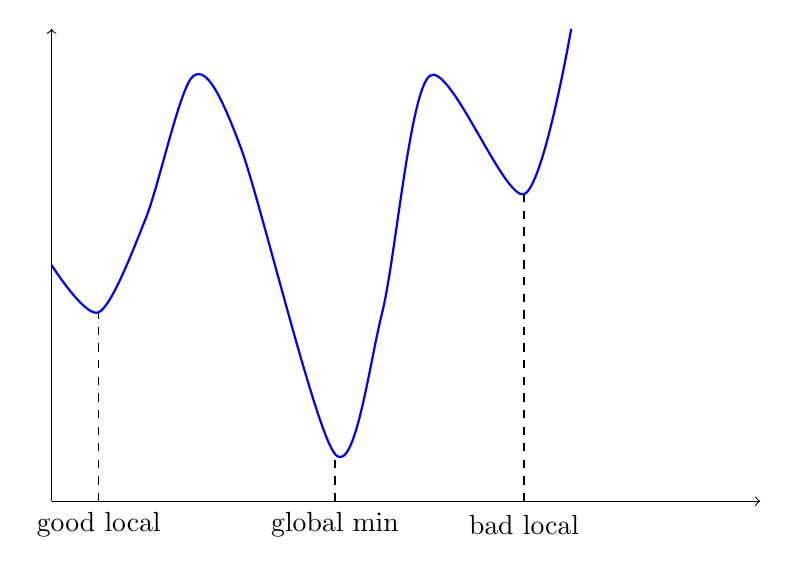
\begin{tikzpicture}[scale=3]
	    \draw[->] (0, 0) -- (3,0);
	    \draw[->] (0, 0) -- (0,2);
	    \draw[thick, blue] plot [smooth, tension=0.5] coordinates{(0, 1) (0.2, 0.8) (0.4, 1.2) (0.6, 1.8) (0.8, 1.5) (1.2, 0.2) (1.4, 0.8) (1.6, 1.8) (2, 1.3) (2.2, 2)};
		\node at (0.2, -0.1) {good local};
		\node at (1.2, -0.1) {global min};
		\node at (2, -0.1) {bad local};
	
		\path 
		(0.2, 0) edge[dashed] (0.2, 0.8)
		(1.2, 0) edge[dashed] (1.2, 0.2)
		(2, 0) edge[dashed] (2, 1.3)
		;
	\end{tikzpicture}
	\caption{Rappresentazione del problema del minimo locale.}
\end{figure}

Per evitare il problema è importante scegliere una configurazione iniziale adeguata dei pesi. Se essi sono troppo elevati la derivata della funzione $g$ sarà vicina a zero e di conseguenza $\Delta w$ avrà valori molto piccoli. In questo modo il rischio di incappare in un minimo locale aumenta. Nella pratica si utilizza la seguente euristica per impostare i pesi iniziali:
\begin{align*}
	w_{ij} \simeq \frac{1}{\sqrt{k_i}}
\end{align*}
dove $k_i$ è il numero di unità entranti nell'unità $i$.

% section problema_del_minimo_locale (end)

% chapter algoritmo_di_back_propagation (end)
